%
% EREORG 5.x User Manual
%
\documentclass[oneside,11pt,openany]{book}
\usepackage{amsmath}
\usepackage{graphicx}
\usepackage[normalem]{ulem}

\pagestyle{myheadings}
\markright{PCET 5.x}
\newcommand{\tw}{\ttfamily}
\makeindex

\begin{document}
%
\title{EREORG User Manual}
%
\author{Alexander Soudackov\\
Ivan Rostov\\
%
\it{\small Department of Chemistry,}\\
\it{\small Yale University,}\\
\it{\small 225 Prospect St,}\\
\it{\small New Haven, CT 06520}}
%
\date{Version 5.4, February 2019}

\maketitle
\frontmatter
%=======================================================================
\chapter*{About PCET}
PCET ({\bf P}roton-{\bf C}oupled {\bf E}lectron {\bf T}ransfer)
is a program package originally developed in the Sharon Hammes-Schiffer
research group at the Department of Chemistry and Biochemistry,
University of Notre Dame by A.~Soudackov, H.~Decornez and I.~Rostov in
the framework of the project "Theoretical Study of Proton-Coupled
Electron Transfer Reactions in Solution" funded by the National Science
Foundation. The package is the property of the Sharon Hammes-Schiffer
research group.

%=======================================================================
\chapter*{Disclaimer}
The developers and maintainers of the PCET package and its offsprings
{\it do not} guarantee that the package is free from err\xout{r}ors. They
{\it do not} accept any responsibility for any loss or damage that
may result from its use. Users are not entitled to redistribute the
program to third parties without consent of the owners.

\tableofcontents

\mainmatter

%=======================================================================
\chapter{Introduction}
EREORG is a utility package (part of PCET) designed to calculate the
reorganization energy matrices using the Ellipsoidal Model (ELCM) or
Frequency Resolved Cavity Model (FRCM) for advanced solvation calculations
in the framework of the dielectric continuum model.

%-----------------------------------------------------------------------
\section{Functionality}

\subsection{General features}

\begin{itemize}

\item Solvent models
\begin{itemize}
\item continuum electrostatic model with ellipsoidal cavity
      \cite{Kirkwood38}
\item advanced continuum Frequency Resolved Cavity Model (FRCM)
      with cavities of molecular shape \cite{Rostov-1}
\end{itemize}

\item Free energy surfaces as functions of scalar solvent
      coordinates (on the grid or along a given path)
\begin{itemize}
\item diabatic and adiabatic free energy curves for single ET
      reaction between any two EVB states
\end{itemize}

\item Rates
\begin{itemize}
\item nonadiabatic rates for a single ET reaction for
      any pair of EVB states
\end{itemize}

\end{itemize}

\subsection{Limitations}

There are two main limitations in the current version of PCET
program:
\begin{itemize}
\item the four-state MS-EVB model is implemented. It means that
      maximum two coupled charge transfer processes can be
      described. Accordingly, four different charge
      distributions in the reacting system should be defined.
\end{itemize}

%-----------------------------------------------------------------------
\section{Programming Language}
All the routines in the current version of PCET are written
mostly in FORTRAN 90. Memory allocation is done using
FORTRAN 90 rules and syntax. FORTRAN 90 features
used in FRCM related routines were removed to maintain
the backward compatibility with the original FRCM code
written in FORTRAN 77.

%-----------------------------------------------------------------------
\section{Target Computers}
Currently, PCET package can be built on the following platforms:
\begin{itemize}
\item Linux (Intel ifort and PGI pgf90 compilers with optional use of Intel MKL libraries)
\item OS X 10.7+ (GNU gfortran compiler)
\end{itemize}

%-----------------------------------------------------------------------
\section{Required External Libraries}
BLAS and LAPACK libraries (MKL libraries for Intel compiler)

%-----------------------------------------------------------------------
\section{Arithmetic Precision}
\begin{itemize}
\item All real variables and parameters are specified as {\tw real(kind=8)}
\item All integer variables are specified as {\tw integer(kind=4)}
\end{itemize}

%-----------------------------------------------------------------------
\section{Units}
The program uses kcal/mol for energy, Angstr\"oms for length, and picoseconds
for time. All the charges and masses are in atomic units.

%-----------------------------------------------------------------------
\section{The REORG directory structure}
\begin{tabular}{ll}
subdirectory & contents \\ \hline
{\tw bin}       & executable and submission scripts \\
{\tw docs}      & documentation (in TeX and PDF formats) \\
{\tw source}    & FORTRAN source files, {\tw Makefile} etc. \\
{\tw tests}     & input and output files for testing \\
\end{tabular}

%=======================================================================
\chapter{Theoretical Background}

%-----------------------------------------------------------------------
\section{Solvation models}
\subsection{Ellipsoidal Model}
In this model the solute is represented by a set of point charges
located on one axis. Different charge distributions corresponding
to VB basis states are modelled by different magnitudes of point
charges. The point charges representing the solute are placed
on the main axis of an axially symmetrical ellipsoidal cavity
embedded in a dielectric continuum solvent characterized by the
inertial ($\epsilon_0$) and electronic (optical) ($\epsilon_\infty$)
dielectric constants (see Fig.~\ref{fig1}).
\begin{figure}[!bbb]
\begin{center}
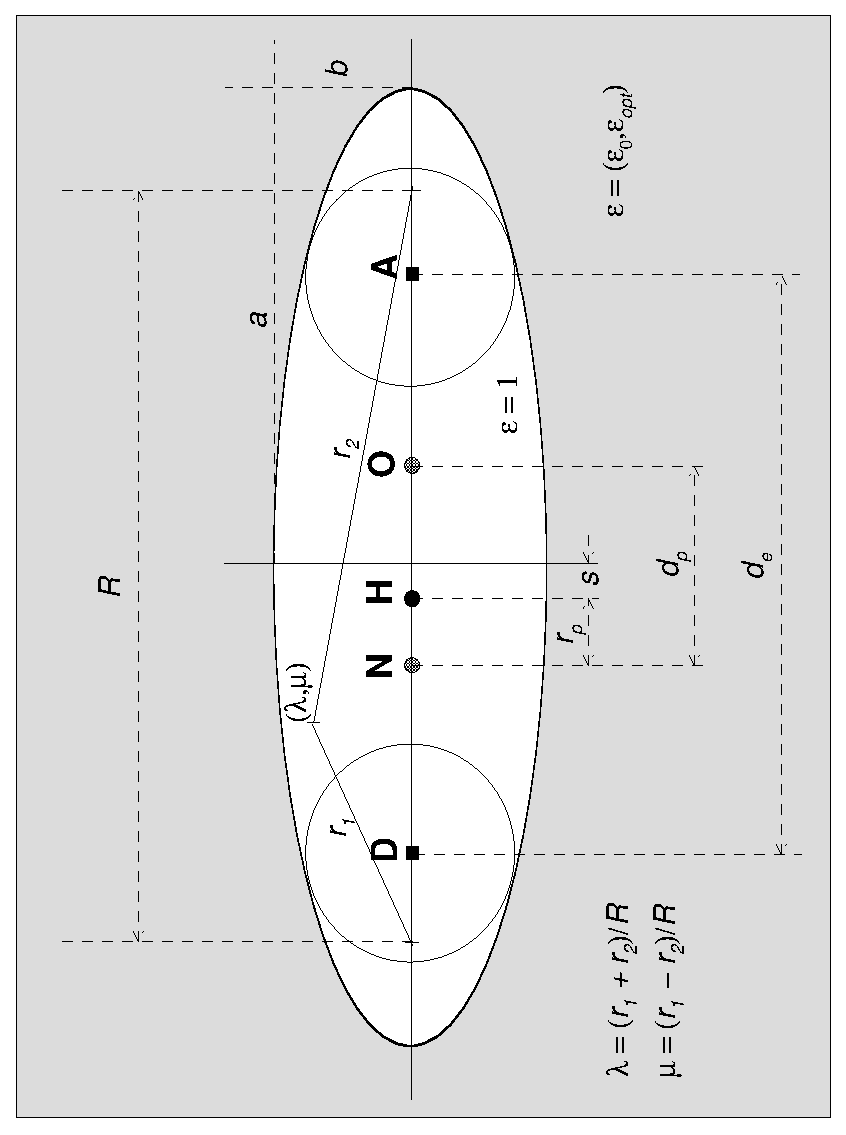
\includegraphics[scale=0.65,angle=-90]{ellips.eps}
\end{center}
\caption{Ellipsoidal model cavity and its geometrical parameters.}
\label{fig1}
\end{figure}
\par
The total polarization potential $\phi(\mu,\lambda)$ at the point ($\mu$,$\lambda$) (elliptical coordinates) inside the cavity
can be expressed as\cite{Kirkwood38}
\begin{equation}
\phi(\mu,\lambda)=\sum_{n=0}^{\infty}B_n(\epsilon_0)P_n(\mu)P_n(\lambda)
\label{phi_tot}
\end{equation}
where $B_n$ are constants and $P_n$ are the Legendre functions
of the first kind. The expression for the coefficients $B_n$
is readily obtained from traditional electrostatics:
\begin{equation}
B_n=\frac{2(2n+1)\beta_n}{R}\left(\frac{1}{\epsilon_0}-1\right)
\frac{Q_n(\lambda_0)}{P_n(\lambda_0)}
\left[1-\frac{1}{\epsilon_0}
\frac{\lambda_0-P_{n-1}(\lambda_0)/P_n(\lambda_0)}
     {\lambda_0-Q_{n-1}(\lambda_0)/Q_n(\lambda_0)}
\right]^{-1}
\label{bcoef}
\end{equation}
Here $R$ is the interfocal distance, $\lambda_0$ defines the
ellipsoid boundary, $Q_n$ are the Legendre functions of the
second kind, and $\beta_n$ is given by the sum over the N
point charges with magnitudes $q_k$ and positions on the axis
$\mu_k$
\begin{equation}
\beta_n=\sum_{k=1}^N q_kP_n(\mu_k)
\label{beta}
\end{equation}
\par
The inertial polarization field is calculated as a difference
between the total field and the electronic polarization field:
\begin{equation}
\phi_{\mathrm in} = \phi - \phi_{\infty}
\label{phi_in}
\end{equation}
where $\phi_{\infty}$ is obtained using
Eqs.(\ref{phi_tot}-\ref{bcoef}) by substituting $\epsilon_0$
in Eq.(\ref{bcoef}) with $\epsilon_{\infty}$.
\par
The reorganization energy matrix elements are calculated
then on the grid along the proton coordinate by using standard definitions\cite{pcet-jcp1}:
\begin{eqnarray}
t_{ij} &=& -\sum_k q_k^{(i)}(\phi^{(j)}-\phi^{(j)}_{\infty}) \\
t_{ij}^{(\infty)} &=& -\sum_k q_k^{(i)}\phi^{(j)}_{\infty}
\label{tmat}
\end{eqnarray}
where indices $i$ and $j$ label charge distributions corresponding
to the VB basis states.


\subsection{FRCM}

Relevant references:
\begin{itemize}
\item{Chudinov, Napolov, and Basilevsky, Chemical Physics {\bf 160}, 41-54 (1992).}
\item{
Basilevsky, Rostov, and Newton, Chemical Physics {\bf 232}, 189-199 (1998).}
\item{
Soudackov and Hammes-Schiffer, J. Chem. Phys. {\bf 111}, 4672 (1999).}
\end{itemize}
\section*{Description of algorithm}
\subsection*{Reorganization energy matrix elements}
The multistate continuum theory requires the calculation
of the solvent
reorganization energy matrix elements defined as
\begin{equation}
t_{ij}=-\int d{\bf r}\, \rho_i \hat{\cal{K}}_{\mathrm{in}} \rho_j
= -\int d{\bf r}\, \rho_i \phi_j^{\mathrm{(in)}},\,\,\, \phi_j^{\mathrm{(in)}}=\hat{\cal{K}}_{\mathrm{in}} \rho_j
\end{equation}
and
\begin{equation}
t_{ij}^{(\infty)}=-\int d{\bf r}\, \rho_i \hat{\cal{K}}_{\infty} \rho_j
= -\int d{\bf r}\, \rho_i \phi_j^{(\infty)},\,\,\, \phi_j^{(\infty)}=\hat{\cal{K}}_{\infty} \rho_j.
\end{equation}
Here the operator $\hat{\cal{K}}_\infty=\hat{\cal{K}}(\epsilon_\infty)$
and $\hat{\cal{K}}_{\mathrm{in}}=\hat{\cal{K}}(\epsilon_o)-
\hat{\cal{K}}(\epsilon_\infty)$,
where $\hat{\cal{K}}(\epsilon)$ is a dielectric Green
function for the medium with dielectric constant $\epsilon$ and
$\epsilon_o$ and $\epsilon_\infty$ are the static and
electronic dielectric constants, respectively.
The calculation of these reorganization energies
requires the calculation of the potentials
$\phi_j^{(\infty)}=\hat{\cal{K}}(\epsilon_\infty) \rho_j$ and
$\phi_j^{\mathrm{(tot)}} = \hat{\cal{K}}(\epsilon_o) \rho_j$
caused by the charge density $\rho_j$ in a dielectric continuum
with dielectric constant $\epsilon_\infty$ and $\epsilon_o$, respectively.
The inertial potential may be calculated from these
two potentials: 
\begin{equation}
\phi_j^{\mathrm{(in)}}=\phi_j^{\mathrm{(tot)}}
- \phi_j^{\mathrm{(\infty)}}.
\label{eq.phiin}
\end{equation}
The FRCM method is used to calculate these potentials.
%
\subsection*{Calculation of the electrostatic potential due to solvent response}
%
The standard PCM method is used to calculate the
electronic solvent potential $\phi_j^{(\infty)}$.
In this method,
the entire charge density $\rho_j$ is placed in a
cavity of arbitrary shape with surface $S$.
The dielectric
constant is equal to unity
inside the cavity and is equal to $\epsilon_\infty$
outside the cavity.
The electronic solvent potential $\phi_j^{(\infty)}$ is calculated by solving
the Poisson equation
with the appropriate boundary conditions at the surface of the
cavity.
(Note that the total potential used in the Poisson
equation is the sum of the potential
due to the charge density $\rho_j$ in a vacuum
and the solvent potential $\phi_j^{(\infty)}$ describing 
the potential due to the solvent response to the density $\rho_j$.)
The solvent potential 
may be expressed in terms of a surface charge density $\sigma_j$
on the surface $S$.  Thus, the problem is reduced to
the calculation of
this surface charge density $\sigma_j$ corresponding
to the charge density $\rho_j$.
The surface charge density $\sigma_j$ may be defined
in terms of a standard integral equation, which must
be solved iteratively.  
\par
The FRCM method is used to calculate the
total solvent potential $\phi_i^{\mathrm{(tot)}}$.
In this method,
two cavities are formed around the charge density $\rho_j$.  
This leads to an inner
surface $S_1$ and an outer surface $S_2$.
The entire charge density is assumed to be
contained inside the inner cavity.
The dielectric constant is equal to unity inside
the inner cavity, to $\epsilon_\infty$ in the
region between the two surfaces $S_1$ and $S_2$, and to $\epsilon_o$
in the region outside the outer cavity.
The solvent potential $\phi_j^{\mathrm{(tot)}}$ is calculated by solving
the Poisson equation
with the appropriate boundary conditions at the two surfaces
$S_1$ and $S_2$.
(Again, note that the total potential used in the Poisson
equation is the sum of the potential
due to the charge density $\rho_j$ in a vacuum
and the solvent potential $\phi_j^{\mathrm{(tot)}}$ describing 
the potential due to the solvent response to the density $\rho_j$.)
The solvent potential 
may be expressed in terms of two surface charge distributions
$\sigma_j^{(1)}$ and $\sigma_j^{(2)}$ on the surfaces $S_1$ and $S_2$, 
respectively.
In this case, the problem requires
the calculation of
both surface charge distributions corresponding
to the charge density $\rho_j$.
These surface charge densities may be defined
in terms of integral equations which must
be solved iteratively.  
\par
In order to numerically solve
the integral equations for both PCM and FRCM, the
surface integrals are computed
by dividing the surface into small pieces.  
These surface
elements are denoted ``tesserae" or  ``sectors" (where the terms
are used interchangably, although a
sector actually refers to a three-dimensional segmenet
and a tesserae actually refers to only the surface element).
The convergence of the iterative solution of the Poisson equation is
determined by the dimensionless parameter SELFCR, where
the convergence criterion is defined to be SELFCR$\times 10^{-4}$
for the outer cavity and SELFCR$\times 10^{-5}$ for the inner cavity.
The default is SELFCR=2.0.  In past versions, the keyword PRECISE 
decreases this to SELFCR=0.2, but
this word should not be used in the current version.
After the surface charge density has converged, it is
renormalized according to the total charge of the solute.
If the total surface charge computed from the
numerical surface charge density differs from the value
determined by the total solute charge
by more than CHDIFF directly prior to the renormalization
of the surface charge density, an error message
is printed.  The default value
is CHDIFF=0.1.
The maximum number of iterations is ITSE, after which an
error message is printed and the program is stopped.
The default value is ITSE=15.
\par
Thus, the calculation of the electronic and inertial
potentials requires the following steps:
\begin{enumerate}
\item{Generate the surfaces of the two cavities.}
\item{Generate the tesserae independently for the two cavities.}
\item{Numerically solve the Poisson equation using PCM for the inner
cavity surrounded by solvent with dielectric constant $\epsilon_\infty$
to obtain the electronic potential $\phi_j^{(\infty)}$.}
\item{Numerically solve the Poisson equation using FRCM for the two cavities
with solvent of dielectric constant $\epsilon_\infty$ in between
the two surfaces and $\epsilon_o$ outside both cavities
to obtain the total potential $\phi_j^{\mathrm{(tot)}}$.}
\item{Calculate the inertial
potential $\phi_j^{\mathrm{(in)}}=\phi_j^{\mathrm{(tot)}}
- \phi_j^{(\infty)}$.}
\item{Use these potentials to calculate the electronic
and inertial reorganization energy matrix elements.}
\end{enumerate}
%
\subsection*{Generation of surfaces}
%
In FRCM, the inner cavity is generated by placing
a sphere centered on each atom with radius $\kappa r_{vdw}$,
where $r_{vdw}$ is the van der Waals radius for the specific atom
and $\kappa$ is independent of the solvent
with a default value of 0.9.
In the FRCM program, the surface of the inner cavity
may be smoothed by including additional spheres.
The key words SMOOTH and NOSMOOTH denote cavity smoothing
or the absence of cavity smoothing.  The default is to include
smoothing.  
The parameter SOLRD defines the effective radius (in Angstroms) of the solvent
molecules and is used to calculate the excluded volume at the
seam of a pair of overlapping spheres.
The default value is SOLRD=1~\AA.
The parameter EXVOL defines
the minimum excluded volume (in cubic Angstroms) at such a seam
for which an auxiliary sphere is
added during smoothing.  The default value is EXVOL=1~\AA$^{3}$.
If EXVOL (or SOLRD) is large enough, the effect is the same as
using the key word NOSMOOTH.
The outer sphere cavity is generated by adding
$\delta$ to the radius of each sphere used to create
the inner cavity (including the spheres added for smoothing).
In general, $\delta$ depends on the solvent.
%
\subsection*{Generation of tesserae/sectors}
%
The premise of the method for generation of the tesserae (or sectors)
is that the surface charges
change more rapidly closer to the seam of the intersection
between two spheres.  Thus, the surface elements should be
chosen to be smaller in the regions of close contact of the spheres.
The following three steps are used to generate the tesserae.
\begin{enumerate}
\item{The first step
is to create a network of A-sectors for each pair of spheres.  
These sectors
are smaller in contact regions (i.e., where the spheres overlap) and larger
in regions near the poles.
The tesserae are created through a series
of rings moving from a contact region to a pole.
The tesserae (or sectors) are defined in terms of
the standard polar angles $\theta$ and $\phi$, where
$0<\theta<180^o$ and $0<\phi<360^o$, and $\theta$
is measured relative to the axis connecting the centers of the pair
of spheres.  The parameters that determine the sizes of the A-sectors
and the basic procedure used to create the A-sectors
are as follows.
\begin{itemize}
\item{The parameters that determine the sizes of the A-sectors
are MODFE1 and MODFE2 for the inner and outer surfaces,
respectively.  
This discussion will use MODFE1 as the example.
The maximum angular step size $\Delta \theta$ for $\theta$ is defined
as 
\begin{equation}
N=400/3/\mbox{MODFE1}.
\end{equation}
For the default value of MODFE1=6, $N=22.2^o$.
The first two rings near the contact region have
$\Delta \theta=0.6N$ and $\Delta \theta =0.9N$, respectively, and the remaining
rings have $\Delta \theta= N$.
The values for these angular step sizes are stored in the
array DDTET, where the first element is $0.6N$,
the second element is $0.9N$, and the remaining elements are $N$.
The number of elements is such that the sum of all angles
is less than 180$^o$.  Thus, for MODFE1=6,
DDTET=(13.3, 20.0, 22.2, 22.2, 22.2, 22.2, 22.2, 22.2).
The angle $\phi$ has the same angular step size $\Delta \phi$ as $\theta$
except for the first two rings, where $\Delta \phi=1.33 \Delta \theta$
and $\Delta \phi=1.28 \Delta \theta$, respectively.}
\item{
The A-sectors are created for each pair in the following manner.
First, the angle in $\theta$ for the overlap between the spheres
is determined to exclude it from consideration.
Second, the sectors are created through a series of rings, using
the angular step sizes from the array DDTET,
starting at the contact
region and moving toward the pole.
The sectors are renormalized to render the total sum of
angular steps
for $\theta$ and $\phi$ $180^o$ and $360^o$, respectively.
Since this procedure is done for each pair of spheres,
for each sphere there is a combination of overlapping
networks of A-sectors due to all of its neighbors.}
\item{
The relation between MODFE1 and MODFE2 is critical to the numerical
accuracy.  Typically, for MODFE1=MODFE2, the number of
tesserae is significantly greater for the inner surface than
for the outer surface.
This results from the greater overlap between the larger spheres
for the outer surface, leading to a larger value of the
excluded angle $\theta$ and thus to a smaller number
of tesserae for each pair of spheres.  In addition,
the spheres added for smoothing  of the inner surface do not
contribute as much to the surface area of the outer cavity.
Furthermore, for MODFE1=MODFE2,
the tesserae are larger in surface area for the
outer surface than for the inner surface.
This inconsistency between the size and
number of tesserae on the two surfaces leads to numerical
instabilities.
One approach is to choose MODFE2 
such that the maximum area of the tesserae for the
inner and outer surfaces is approximately equal.  This
can be achieved using the equation
\begin{equation}
\mbox{MODFE2}=\mbox{MODFE1}*(\kappa r_{vdw}+\delta)/(\kappa r_{vdw})
\end{equation}
for a typical value of $r_{vdw}$ for the system of interest.
Another approach is to choose MODFE2 such that the number
of tesserae on the inner and outer surfaces is nearly equal.
}
\end{itemize}}
\item{
The second step 
to create a network of small elements, called
B-sectors.  These are also defined in terms of the angles $\theta$ and
$\phi$.
The angular step sizes are defined
in terms of NTETFI1 and NTETFI2 for the inner and outer cavities,
respectively.  This discussion will use NTETFI1 as the example.
The angular step sizes are defined as
\begin{eqnarray}
\Delta \phi &=& 360/(\mbox{NTETFI1} * 120) \\
\Delta \theta &=& 180/(\mbox{NTETFI1} * 60).
\end{eqnarray}
The default is NTETFI1=NTETFI2=1, which leads to step sizes of 3$^o$.
This leads to 7200 B-sectors per sphere.}
\item{
In the third step of the generation of the tesserae, 
the A-sectors and the B-sectors are used to construct a unique
set of sectors completely covering the whole surface, called
the C-sectors.  In this procedure, each B-sector is
related to the A-sector derived from the neighboring sphere
closest to it.  Thus, each B-sector is uniquely related
to an A-sector.  The B-sectors related to
the same A-sector are combined as a cluster
called a C-sector.  The network of C-sectors
completely and uniquely covers the cavity surface.
In order to decrease the total number of C-sectors,
some of the C-sectors are combined with neighboring smaller ones.}
\end{enumerate}


%=======================================================================
\chapter{Compiling and Execution}
%-----------------------------------------------------------------------
\section{Compiling EREORG}
To compile EREORG program for a specific platform you need
change to the {\tw source} directory, then
copy or link {\tw Makefile.xxx} to {\tw Makefile.machine}, for example

\begin{description}
\item {\tw ln -s Makefile.xxx Makefile.machine}
\item {\tw make all}
\end{description}

\noindent where {\tw <xxx>} must be substituted by
the platform-specific suffix. With the present version only one
makefile is supplied:
\par\noindent
\begin{tabular}{lcp{8cm}}
{\tw Makefile.gfortran} &-& for GFORTRAN compiler \\
{\tw Makefile.lnx} &-& for LINUX platforms with Portland
      Group FORTRAN compiler {\tw pgf77} \\
\end{tabular}

This will initiate compiling and linking of the program. First,
the makefile will build an object library containing all the object
files except the object file for the main program. Then the
makefile will combine the main object file with the library
and produce the executable {\tw reorg\_frcm\_<x.x>\_gfortran.x} which will
be placed in the {\tw bin} directory.

When you modify the include files with parameters and array
dimensions, you {\bf must} recompile all the source codes
and build a new library. To remove the old object library
run the command

\begin{description}
\item {\tw make clean}
\end{description}


%-----------------------------------------------------------------------
\section{Running EREORG}

You can run EREORG program from any directory you wish provided
that the path to the executable is listed in your {\tw PATH}
variable or you have a link to the executable in your current
directory.

You will need two mandatory (and maybe more optional) input files
in your current directory. The main input file (control file)
with arbitrary name contains the control information
(keywords) about the jobs you want to run. It contains
also the names of other optional input files you may
want to use. The other mandatory file is the file
with geometry specification for solvation
calculations. The name of this file is
specified in the keyword section of the control input file.
The detailed information about the structure of the input
files is given in the next chapter.

To initiate execution you have to run the command

\begin{description}
\item {\tw reorg\_frcm\_<x.x>\_gfortran.x <name-of-the-control-input-file>}
\end{description}

The program will generate a screen output (you might want to
redirect it to disk using standard redirection rules) and
also other optional output files which will be placed
in the new subdirectory with the name specified in the title
section of the control input file.


%=======================================================================
\chapter{Structure of the DATA Files}

%-----------------------------------------------------------------------
\section{Control Input File}

\subsection{General structure}
The control input file consists of blocks separated by
empty lines. Each block contains the control information
for a particular job. The program reads blocks sequentially
and terminates when it finds the word {tw END} in the
beginning (first three positions) of the block. All the
lines in the control input file must be not longer
than 80 symbols. The symbols after first 80 are ignored.

Each block consists of three sections:
\begin{enumerate}
\item TITLE SECTION (one line) -
      the title of the job and optionally the keyword
      specifiyng the name of the job. This keyword
      has the following format: {\tw JOBNAME=<name-of-the-job>}.
      If this keyword is specified the program will
      create a subdirectory {\tw name-of-the-job}
      for optional output files. Otherwise a subdirectory
      with the standard name (consequtive number of the job)
      will be created.

\item COMMENT SECTION (one line) -
      any text specifying the current job

\item KEYWORDS SECTION (as many lines as you want but the total
      number of symbols should not exceed 480) - the keywords
      controlling the job. The detailed description of all
      the keywords and related options is given in the next
      subsection.

\end{enumerate}

\subsection{Keywords}
There are two types of keywords in the PCET 2.0 program. The keywords
of the first type set some global controls for the job and are
mandatory. The keywords of the second type provide the control
information about specific tasks which should be performed.
Usually these keywords require mandatory set of options given
in brackets. The format for the first type of keywords is
(no spaces before or after "="!)

\begin{description}
\item {\tw KEYWORD=<value>}
\end{description}

\noindent The format for the second type is (no spaces before
the opening bracket!)

\begin{description}
\item {\tw KEYWORD(Option1,Option2,Option3,...)}
\end{description}

\noindent The keywords are case-insensitive and should be separated
by spaces. The options are separated by commas and are case-insensitive
as well.

Below is the list of keywords with detailed descriptions.

%\subsubsection*{CHARGE=$Q$}
%
%Sets the total charge of the solute $Q$ (a.u.).

\subsubsection*{SOLV({\it Options})}
%
Defines the model and parameters for solvation calculations.
The available option are:
%
\begin{description}
\item[{\tw WATER}] - the solvent is water
\item[{\tw H2O}] - the solvent is water
\item[{\tw CH2CL2}] - the solvent is methylene chloride (dichloromethane)
\item[{\tw MEOH}] - the solvent is methanol
\item[{\tw ETOH}] - the solvent is ethanol
\item[{\tw CH3CN}] - the solvent is CH$_3$CN
\item[{\tw DCE}] - the solvent is DCE
\item[{\tw THF}] - the solvent is THF (tetrahydrofurane)
\item[{\tw NBZ}] - the solvent is nitrobenzene
\item[{\tw DMF}] - the solvent is DMF
\item[{\tw EPS0=$\epsilon_0$}] - static dielectric constant
\item[{\tw EPS8=$\epsilon_\infty$}] - optical (electronic) dielectric
constant
\item[{\tw ELLIPSE}] - simple electrostatic ellipsoidal model will be used
\item[{\tw A=$a$}] - major semiaxis of the ellipsoidal cavity
\item[{\tw B=$b$}] - minor semiaxis of the ellipsoidal cavity
\item[{\tw FRCM}] - advanced FRCM model will be used
\item[{\tw KAPPA=$\kappa$}] - factor for VdW radii
\item[{\tw DELTA=$\delta$}] - thickness of the inner layer in FRCM
\item[{\tw GEOM=<file>}] - the geometry and EVB charges are given
in the external file {\tw <file>} (the format of the file
is described in the next section).
\item[{\tw TREAD=<file>}] - the reorganization energy matrices
on the grid are read from external binary file {\tw <file>}
saved in previous calculation.
\item[{\tw TWRITE=<file>}] - the reorganization energy matrices
on the grid are saved in the external binary file {\tw <file>}.
\item[{\tw XYZOUT=<file>}] - the cartesian coordinates
are written to the external file {\tw <file>} in XYZ format.
\item[{\tw NOSYMD}] - the reorganization energy martices are not 
about the diagonal from top left to bottom right.  This keyword
should only be used to check how good the approach is working.  By 
default the reorganization energy matrices will be symmetrized.
(See solint.f and tmat.f)
\item[{\tw SYMT}] - the solvent reorganization energy martices are
symmetrized so that the properties for a symmetric PCET system are
correctly reproduced.
\item[{\tw SYMET}] - the solvent reorganization energy martices are
symmetrized so that the properties for a symmetric ET system are
correctly reproduced. (NOTE, this should only be used with the ET2
keyword.
\item[{\tw SYMPT}] - the solvent reorganization energy martices are
symmetrized so that the properties for a symmetric PT system are
correctly reproduced. (NOTE, this should only be used with the PT2
keyword.             
\item[{\tw REDDENS}] - All the elements of the solvent reorganization
energy martices which depend on 2b are obtained from all the other
elements depending only on 1a,1b,2a.  This should always be true anyway.  
A system for which this is not true has some major problems and should
be used with caution. This keyword can also be used when the
charges for the 2b state for solvation are not obtainable.  (simply
put in any charges that are not all zero 
and such that the column has at least 
one different element from the other columns:1a,1b,and 2a.)
\end{description}

\subsubsection*{EREORG({\it Options})}
%
Calculates [4x4] reorganization energy matrices for four given
charge distributions. Also calculates one-dimensional free energy curves
and nonadiabatic rate for a single ET reaction between specified EVB states.
The available options are:

\begin{description}

\item[{\tw REAC=<N>}] - the EVB state {\tw N} (1/2/3/4) will be considered
           as a reactant state in the ET reaction. If this
           option is not specified then the state 1 (1a)
           is assumed to be the reactant state.

\item[{\tw PROD=<M>}] - the EVB state {\tw M} (1/2/3/4) will be considered
           as a product state in the ET reaction. If this
           option is not specified then the state 3 (2a)
           is assumed to be the product state.

\item[{\tw ZE1=<ZE1>}] - the left limit on the grid along the solvent
            coordinate $z_e$ (kcal/mol). The default is
            $-3\lambda_{ET}$, where $\lambda_{ET}$ is the
            ET reorganization energy.

\item[{\tw ZE2=<ZE2>}] - the right limit on the grid along the solvent
            coordinate $z_e$ (kcal/mol). The default is
            $+3\lambda_{ET}$, where $\lambda_{ET}$ is the
            reorganization energy.

\item[{\tw NZE=<N>}] - number of points along the grid. The default is 100.

\item[{\tw EBIAS=<E>}] - the gas phase bias (kcal/mol) for the ET pair. The default is 0.

\item[{\tw VEL=<E>}] - electronic coupling (kcal/mol) for the ET pair. The default is 0.

\item[{\tw PLOT=<filename>}] - name of the output file with the free energy
                  profiles (the default filename is {\tw et.dat}).

\item[{\tw RATE=<T>}] - the nonadiabatic rate at $T=${\tw <T>} K
                        will be calculated. The default temperature
                        is 298.15 K.

\end{description}


%-----------------------------------------------------------------------
\section{Additional INPUT Files}
%
\subsection{Geometry and charges specification}
This input file specifies the geometry and basis EVB point charge
distributions for solvation calculations. The examples are stored
in the {\tw tests} subdirectory as files with
{\tw .sol} extensions.
%
\subsubsection*{Line 1: Keywords}
One keyword is mandatory and defines the format for the geometry
specification. You should specify either {\tw XYZ}
(cartesian coordinates) or {tw INT} (internal coordinates).
If the file is intended for FRCM solvation calculations,
you can also specify any FRCM keywords described in the FRCM
manual.

\subsubsection*{Line 2 - Title}
Any title specifying the geometry.

\subsubsection*{Line 3 - Comment}
Any text related to geometry (can be empty).

\subsubsection*{Lines 4:N - Geometry specification}
The geometry can be specified either in cartesian coordinates
({\tw <element\_symbol>  <x>   <y>   <z>}) or in internal
coordinates ({\tw MOPAC} Z-matrix format). The allowed
element symbols are H-No and also symbols
'De', 'Ae', 'Dp', 'Ap', 'Ps' for general electron donor,
electron acceptor, proton donor, proton acceptor,
and pseudoatom, respectively. Format is free
and the section is terminated by an empty line.

\subsubsection*{Line N+2 - Title for charge distribution section}
Any title specifying the EVB charges (must contain {\tw CHARGES} keyword).

\subsubsection*{Line N+3:M - Charges for EVB states}
Four columns in free format, the columns specify charges
on atoms for EVB states 1a, 1b, 2a, and 2b, respectively.
Note that the order of point charges should exactly
correspond to the order of atoms in the geometry section.
The input of charges is also terminated by an empty line.
{\bf IMPORTANT: the first line in this section should contain TOTAL
charges corresponding to each EVB state}.


%-----------------------------------------------------------------------
\section{OUTPUT Files}
%
\subsection{Standard output}
Standard unit 6 is used for standard output throughout the program.
You can redirect the standard output to the disk file using standard
redirection rules for your operating system.

\subsection{Geometry output}
The program can produce the geometry files if the {\tw XYZOUT} option
is specified with the {\tw HGAS} or {\tw SOLV} keywords. The files are
written in standard "xyz" format, so you can use any vizualization
software to check the geometry (for example, MOLDEN).


%=======================================================================
%
\begin{thebibliography}{99}

\bibitem{pcet-jcp1} A.~V. Soudackov and S. Hammes-Schiffer,
J. Chem. Phys. {\bf 111},  4672 (1999).

\bibitem{pcet-jacs} A.~V. Soudackov and S. Hammes-Schiffer,
J. Am. Chem. Soc. {\bf 121}, 10598 (1999).

\bibitem{pcet-jcp2} A.~V. Soudackov and S. Hammes-Schiffer,
J. Chem. Phys. {\bf 113},  2385 (2000).

\bibitem{pcet-jpc} H.~Decornez, S.~Hammes-Schiffer,
Model proton-coupled electron transfer reactions in solution:
Predictions of rates, mechanisms, and kinetic isotope effects,
J.~Phys.~Chem.~A. (in press)

\bibitem{voth-schmitt} U.~W.~Schmitt, G.~A.~Voth,
J.~Phys.~Chem. B{\bf 102}, 5547 (1998)

\bibitem{Kirkwood38}
F.~H.~Westheimer, J.~G.~Kirkwood, J. Chem. Phys. {\bf 6}, 513 (1938)

\bibitem{Rostov-1}
M.~V. Basilevsky, G.~E. Chudinov, I.~V. Rostov, Y.-P. Liu, and M.~D. Newton,
  Journal of Molecular Structure {\bf 371},  191  (1996).

\bibitem{Webb-DFGH} S.~P.~Webb, S.~Hammes-Schiffer,
Discrete Fourier grid multiconfigurational self-consistent-field:
A method to calculate multidimensional hydrogen vibrational wavefunctions,
J.~Chem.~Phys. (in press)

\end{thebibliography}


\end{document}
